\documentclass[spanish]{beamer}
\usepackage[utf8]{inputenc}
\usepackage{float}
\usepackage{beamerthemesplit}
\usepackage{latexsym}
\usepackage[T1]{fontenc}
\usepackage{amsmath}
\usepackage{hyperref}
\usepackage{graphicx}
\usepackage{babel,blindtext}
\usepackage{amsfonts}
\usepackage[round]{natbib}
\bibliographystyle{chicago}
\usepackage{subcaption} 


\decimalpoint

\usetheme{Antibes}%este es el templete que se usa a lo largo de la presentacion
%themes
%   default
%   Boadilla
%   Madrid
%   Pittsburgh
%   Copenhagen
%   Warsaw
%   Singapore
%   Malmoe
\newcommand\Fontvi{\fontsize{6}{7.2}\selectfont}
\mode<presentation>%tipo de 
\begin{document}

%%%%%%%%%%%%%%%%%%%%%%%%%%%%%%%%%%%%%%%%%%%%%%%%%%%%%%%%%%%%%%%%%%%%%%%%%%%%%%%%%%%%%%%%%%%%%%%%%%%%%%%%%%%%%
\title{Markov Chains}
\author{Gamaliel Moreno Chávez}
\institute{MCPI}
\date{Ago-Dic\\ 2020}%para que ponga la fecha de hoy 

\frame{\titlepage}
%%%%%%%%%%%%%%%%%%%%%%%%%%%%%%%%%%%%%%%%%%%%%%%%%%%%%%%%%%%%%%%%%%%%%%%%%%%%%%%%%%%%%%%%%%%%%%%%%%%%%%%%%%%%%
%%%%%%%%%%%%%%%%%%%%%%%%%%%%%%%%%%%%%%%%%%%%%%%%%%%%%%%%%%%%%%%%%%%%%%%%%%%%%%%%%%%%%%%%%%%%%%%%%%%%%%%%%%%%%%%%%%%%%%%%%%%%%%%%%%%%%%%%%%%%%%%%%%%%%%%%%%%%%%%%%%%%%%%%%%%%%%%%%%%%%%%%%%%%%%%%%%%%%%%%%%%%%%%%%%%%%%%%%%
%%%%%%%%%%%%%%%%%%%%%%%%%%%%%%%%%%%%%%%%%%%%%%%%%%%%%%%%%%%%%%%%%%%%%%%%%%%%%%%%%%%%%%%%%%%%%%%%%%%%%%%%%%%%%%%%%%%%%%%%%%%%%%%%%%%%%%%%%%%%%%%%%%%%%%%%%%%%%%%%%%%%%%%%%%%%%%%%%%%%%%%%%%%%%%%%%%%%%%%%%%%%%%%%%%%%%%%%%%

\begin{frame}
\frametitle{Introducción}
\begin{center}
{\huge ¿cuál es la característica principal de un procesos Markoviano?}
\end{center}

 
\end{frame}

%%%%%%%%%%%%%%%%%%%%%%%%%%%%%%%%%%%%%%%%%%%%%%%%%%%%%%%%%%%%%%%%%%%%%%%%%%%%%%%%%%%%%%%%%%%%%%%%%%%%%%%%%%%%%
\begin{frame}
\frametitle{Estados y transiciones} 
Cadenas de Markov
\begin{itemize}
\item Secuencia de paso o intentos discretos numerados por $n=0,1,2,\ldots$
\item El resultado de n-th intento es la variable aleatoria $X_{n}$
\item $X_{0}$ es la posición inicial de proceso. Esta variable aleatoria puede tomar valores $i=1,2,\ldots, m$ 
\item El resultado actual es llamado estado del sistema y se donota como $E_{i} (i=1,2,\ldots, m)$
\end{itemize}
\footnotetext[1]{La caminata aleatoria es un caso especial de un proceso más general, el de Markov .}
´\end{frame}
%%%%%%%%%%%%%%%%%%%%%%%%%%%%%%%%%%%%%%%%%%%%%%%%%%%%%%%%%%%%%%%%%%%%%%%%%%%%%%%%%%%%%%%%%%%%%%%%%%%%%%%%%%%%%
\begin{frame}
\frametitle{Estados y transiciones}
Cadenas de Markov

Si la v.a.s $X_{n-1} = i$ y $X_{n} = j$, entonces el sistema ha realizado un transición $E_{i} \rightarrow E_{j} $, esto es, una transición del estado $E_{i}$ al estado $E_{j}$ en el intento n-th.

Notese que $i$ puede ser igual que $j$, las transiciones al mismo estado son posibles.
La asignación de potabilidades a las transiciones de $E_{i} \rightarrow E_{j}$ es conocida como cadena

\end{frame}
%%%%%%%%%%%%%%%%%%%%%%%%%%%%%%%%%%%%%%%%%%%%%%%%%%%%%%%%%%%%%%%%%%%%%%%%%%%%%%%%%%%%%%%%%%%%%%%%%%%%%%%%%%%%%
\begin{frame}
\frametitle{Cadenas de Markov}
Las cadenas de Markov tiene la propiedad de que la probabilidad de que $X_{n}=j$ depende solamente del estado previo del sistema.  Formalmente, esto significa que no necesitamos más información en cada paso que, para cada i y j.


\begin{multline*}
P\lbrace X_{n} = j\vert X_{n-1} = i\rbrace = P\lbrace X_{n} = j\vert X_{n-1} = i, X_{n-1} = K_{n-1},\\ X_{n-2} =  K_{n-2}, \ldots X_{1} = K_{1} \rbrace
\end{multline*}
lo que  significa que la probabilidad $X_{n} = j$ dado $X_{n-1} = i$: es independiente de los valores $X_{n-2} , X_{n-3},  \ldots, X_{1}$. 
\end{frame}

%%%%%%%%%%%%%%%%%%%%%%%%%%%%%%%%%%%%%%%%%%%%%%%%%%%%%%%%%%%%%%%%%%%%%%%%%%%%%%%%%%%%%%%%%%%%%%%%%%%%%%%%%%%%%
\begin{frame}
\frametitle{Cadenas de Markov}
Conceptos básicos
\begin{itemize}
\item Probabilidad de transición 
\item Probabilidad estacionaria o absoluta
\item Probabilidad de transición en $n$ pasos
\end{itemize}
\end{frame}


%%%%%%%%%%%%%%%%%%%%%%%%%%%%%%%%%%%%%%%%%%%%%%%%%%%%%%%%%%%%%%%%%%%%%%%%%%%%%%%%%%%%%%%%%%%%%%%%%%%%%%%%%%%%%
\begin{frame}
\frametitle{Probabilidades de transición}
Para una cadena de Markov finita con $m$ estados $E_{1}, E_{2} ,\ldots, E_{m},$  tenemos 
\begin{equation*}
p_{ij} = P\lbrace X_{n} = j \vert X_{n-1} = i\rbrace,
\end{equation*}

donde $i, j = 1, 2, \ldots, m$  representan las probabilidades de transición del estado $E_{i}$ al $E_{j} $. Las probabilidades $p_{ij}$ son conocidas y cumplen 

\begin{equation*}
p_{ij} \geq 0, \quad \sum_{j=1}^{m}{p_{ij}}=1
\end{equation*}
para cada $i = 1, 2, \ldots, m$. 
\end{frame}
%%%%%%%%%%%%%%%%%%%%%%%%%%%%%%%%%%%%%%%%%%%%%%%%%%%%%%%%%%%%%%%%%%%%%%%%%%%%%%%%%%%%%%%%%%%%%%%%%%%%%%%%%%%%%
\begin{frame}
\frametitle{Probabilidades de transición}
Si $p_{ij}> 0$, entonces decimos que el estado $E_{i}$ puede comunicarse con $E_{j}$, la comunicación es bidireccional si además $p_{ji}> 0$. 

Notese que para cada $i$ fijo, la lista $\lbrace p_{ij}\rbrace$ es una distribución de probabilidad, ya que en cualquier paso de los resultados $E_{1}, E_{2}, \ldots, E_{m}$ debe ocurrir: los estados $E_{i}, (i = 1, 2, \ldots, m)$.
\end{frame}
%%%%%%%%%%%%%%%%%%%%%%%%%%%%%%%%%%%%%%%%%%%%%%%%%%%%%%%%%%%%%%%%%%%%%%%%%%%%%%%%%%%%%%%%%%%%%%%%%%%%%%%%%%%%%
\begin{frame}
\frametitle{Probabilidades de transición}
Las probabilidades de transición forman un arreglo  de $mxm$ el cual puede ser represando por un matriz de transición $T$
\begin{equation}
T =[p_{i,j}]=\begin{bmatrix}
p_{11} & p_{12} & \cdots & p_{1m} \\
p_{21} & p_{22} & \cdots & p_{2m} \\
\vdots & \vdots & \ddots & \vdots \\
p_{m1} & p_{m2} & \cdots & p_{mm} 
\end{bmatrix}
\end{equation} 
Notese que cada renglones de $T$ es una distribución de probabilidad. Cualquier matriz cuadrad para la cual $p_{ij} \geq 0, \sum_{j=1}^{m}{p_{ij}}=1$ se dice que es un renglón estocástico.
\end{frame}
%%%%%%%%%%%%%%%%%%%%%%%%%%%%%%%%%%%%%%%%%%%%%%%%%%%%%%%%%%%%%%%%%%%%%%%%%%%%%%%%%%%%%%%%%%%%%%%%%%%%%%%%%%%%%
\begin{frame}
\frametitle{Probabilidades de transición}
\begin{center}
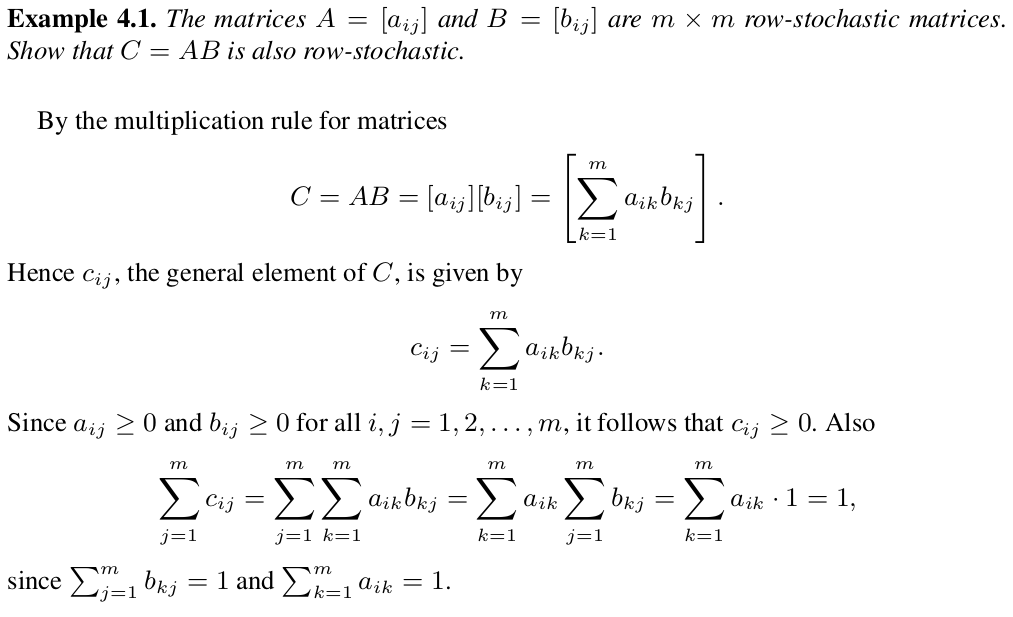
\includegraphics[scale=0.3]{im1}
\end{center}

\end{frame}
%%%%%%%%%%%%%%%%%%%%%%%%%%%%%%%%%%%%%%%%%%%%%%%%%%%%%%%%%%%%%%%%%%%%%%%%%%%%%%%%%%%%%%%%%%%%%%%%%%%%%%%%%%%%%
\begin{frame}
\frametitle{Probabilidad estacionaria o absoluta}
Otra probabilidad de interés es la del el resultado $E_{j}$ después de $n$ pasos, dada una distribución de probabilidad inicial $\lbrace p_{i}^{(0)}\rbrace$.  Donde $p_{i}^{(0)}$ es la probabilidad que inicialmente el sistema ocupe el estado $E_{i}$. Seguro $\sum_{i=1}^{m}p_{i}^{0}=1$. Sea $p_{j}^{(1)}$  la probabilidad de que $E_{j}$ sea ocupado después de un paso. Por la ley de probabilidad total 
\begin{equation*}
p_{j}^{(1)}= \sum_{i=1}^{m}p_{i}^{(0)} p_{ij}
\end{equation*}
podemos expresar $p^{(0)}$ y $p^{(1)}$ esto como dos vectores 
\begin{equation*}
\textbf{p}^{(0)}= \left[ p_{1}^{(0)} p_{2}^{(0)}  \ldots p_{m}^{(0)} \right]  
\end{equation*}

\begin{equation*}
\textbf{p}^{(1)}= \left[ p_{1}^{(1)} p_{2}^{(1)}  \ldots p_{m}^{(1)} \right]  
\end{equation*}


\end{frame}
%%%%%%%%%%%%%%%%%%%%%%%%%%%%%%%%%%%%%%%%%%%%%%%%%%%%%%%%%%%%%%%%%%%%%%%%%%%%%%%%%%%%%%%%%%%%%%%%%%%%%%%%%%%%%
\begin{frame}
\frametitle{Probabilidad estacionaria o absoluta}

La expresión $p_{j}^{(1)}= \sum_{i=1}^{m}p_{i}^{(0)} p_{ij}$ puede ser representada como un producto matricial 


\begin{equation*}
\textbf{p}^{(1)}= \left[ p_{j}^{(1)} \right] = \left[ \sum_{i=1}^{m}p_{i}^{(0)} p_{ij} \right]  =\textbf{p}^{(0)}T´
\end{equation*}


\end{frame}
%%%%%%%%%%%%%%%%%%%%%%%%%%%%%%%%%%%%%%%%%%%%%%%%%%%%%%%%%%%%%%%%%%%%%%%%%%%%%%%%%%%%%%%%%%%%%%%%%%%%%%%%%%%%%
\begin{frame}
\frametitle{Probabilidad estacionaria o absoluta}

Sí $p^{(2)}$ es la distribución después de dos pasos, entonces 

\begin{equation*}
\textbf{p}^{(2)}= \textbf{p}^{(1)} T= \textbf{p}^{(0)}TT = \textbf{p}^{(0)}T^2 
\end{equation*}

por lo tanto después de n pasos de repetir el proceso tenemos 


\begin{equation*}
\textbf{p}^{(n)}= \textbf{p}^{(n-1)} T= \textbf{p}^{(0)}T^{n} 
\end{equation*}
donde

\begin{equation*}
\textbf{p}^{(n)}= \left[ p_{1}^{(n)} p_{2}^{(n)}  \ldots p_{m}^{(n)} \right]  
\end{equation*}

Más generalmente 

\begin{equation*}
\textbf{p}^{(n+r)}=\textbf{p}^{(r)}T^n 
\end{equation*}
\end{frame}
%%%%%%%%%%%%%%%%%%%%%%%%%%%%%%%%%%%%%%%%%%%%%%%%%%%%%%%%%%%%%%%%%%%%%%%%%%%%%%%%%%%%%%%%%%%%%%%%%%%%%%%%%%%%%
\begin{frame}
\frametitle{Probabilidad estacionaria o absoluta}

En $\textbf{p}^{(n)}= \left[ p_{1}^{(n)} p_{2}^{(n)}  \ldots p_{m}^{(n)} \right]  $, el término $p_{j}^{(n)}$ es la probabilidad absoluta o no condicional del resultado $E_{j}$ en el paso $n-th$ dada la distribución inicial $p^{0}$, esto es,
$P \left\lbrace  X_{n}= j \right\rbrace  = p_{j}^{(n)}$. Notese que \begin{equation*}
\sum_{j=1}^{m}{p_{j}^{(n)}}=1
\end{equation*} 
\end{frame}
%%%%%%%%%%%%%%%%%%%%%%%%%%%%%%%%%%%%%%%%%%%%%%%%%%%%%%%%%%%%%%%%%%%%%%%%%%%%%%%%%%%%%%%%%%%%%%%%%%%%%%%%%%%%%

\begin{frame}
\frametitle{Probabilidad estacionaria o absoluta}
Ejercicio. En una cadena de Markov triestado, $E_{1} ,E_{2} ,E_{3}$, cuyo inicio de la cadena es $E_{2}$ de tal manera que la $\textbf{p}^{(0)}= \left[ 0, 1, 0 \right]  $. Encuentre la probabilidad absoluta $\textbf{p}^{(3)}$ si matriz de transición es 

\begin{equation}
T =\begin{bmatrix}
1/2 & 1/4 & 1/4 \\
0 & 1/2 & 1/2  \\
3/4 & 1/4 & 0 
\end{bmatrix}
\end{equation} 
 
\end{frame}

%%%%%%%%%%%%%%%%%%%%%%%%%%%%%%%%%%%%%%%%%%%%%%%%%%%%%%%%%%%%%%%%%%%%%%%%%%%%%%%%%%%%%%%%%%%%%%%%%%%%%%%%%%%%%

\begin{frame}
\frametitle{Probabilidad de transición en el paso-n $p_{ij}^{(n)}$}
Ahora definimos $p_{ij}^{(n)}$ como la probabilidad de que la cadena esté en el estado $E_{j}$ después de $n$ pasos dado que la cadena comenzó en el estado $E_{i}$. Las probabilidades de transición del primer paso $p_{ij} = p_{ij}$ son simplemente los elementos de la matriz de transición $T$. Si tenemos la intención de encontrar una fórmula para $p^{(n)}_{ij}$. Ahora, por definición,
 \begin{equation*}
 p_{ij}^{(n)}=P(X_{n}=j \vert X_{0}=i)
 \end{equation*}
 también 
  \begin{equation*}
 p_{ij}^{(n)}=\sum_{k=1}^{m} P(X_{n}=j, X_{n-1}=k \vert X_{0}=i)
 \end{equation*}
 para $n \geq 2$ ya que la cadena debe haber pasado por uno de todos los m estados posibles en el paso $n-1$.
\end{frame}
%%%%%%%%%%%%%%%%%%%%%%%%%%%%%%%%%%%%%%%%%%%%%%%%%%%%%%%%%%%%%%%%%%%%%%%%%%%%%%%%%%%%%%%%%%%%%%%%%%%%%%%%%%%%%

\begin{frame}
\frametitle{Probabilidad de transición en el paso-n $p_{ij}^{(n)}$}
Ahora definimos $p_{ij}^{(n)}$ como la probabilidad de que la cadena esté en el estado $E_{j}$ después de $n$ pasos dado que la cadena comenzó en el estado $E_{i}$. Las probabilidades de transición del primer paso $p_{ij} = p_{ij}$ son simplemente los elementos de la matriz de transición $T$. Si tenemos la intención de encontrar una fórmula para $p^{(n)}_{ij}$. Ahora, por definición,
 \begin{equation*}
 p_{ij}^{(n)}=P(X_{n}=j \vert X_{0}=i)
 \end{equation*}
 también 
  \begin{equation*}
 p_{ij}^{(n)}=\sum_{k=1}^{m} P(X_{n}=j, X_{n-1}=k \vert X_{0}=i)
 \end{equation*}
 para $n \geq 2$ ya que la cadena debe haber pasado por uno de todos los m estados posibles en el paso $n-1$.
\end{frame}

%%%%%%%%%%%%%%%%%%%%%%%%%%%%%%%%%%%%%%%%%%%%%%%%%%%%%%%%%%%%%%%%%%%%%%%%%%%%%%%%%%%%%%%%%%%%%%%%%%%%%%%%%%%%%

\begin{frame}
\frametitle{Probabilidad de transición en el paso-n $p_{ij}^{(n)}$}
Para tres eventos cualesquiera $A,B,$ y $C$, tenemos la siguiente identidad 
\begin{equation*}
P(A \cap B \vert C) = P(A \vert B \cap C) P(B \vert C) 
\end{equation*} 
Interpretando $A$ como $X_n = j$, $B$ como $X_{n-1} = k$, and $C$ as $X_{0} = i$, queda como sigue 
\small
\begin{align*} 
p_{ij}^{(n)}& = P(A \cap B \vert C) = P(X_{n}=j, X_{n-1}=k \vert X_{0}=i) \\
& =\sum_{k=1}^{m}
(X_{n}=j\vert X_{n-1}=k,  X_{0}=i) P(X_{n-1}=k \vert X_{0}=i)\\
& =\sum_{k=1}^{m}P(X_{n}=j\vert X_{n-1}=k) P(X_{n-1}=k \vert X_{0}=i)\\
& =\sum_{k=1}^{m} p_{kj}^{(1)}p_{ik}^{n-1}
\end{align*}

\end{frame}

%%%%%%%%%%%%%%%%%%%%%%%%%%%%%%%%%%%%%%%%%%%%%%%%%%%%%%%%%%%%%%%%%%%%%%%%%%%%%%%%%%%%%%%%%%%%%%%%%%%%%%%%%%%%%

\begin{frame}
\frametitle{Probabilidad de transición en el paso-n $p_{ij}^{(n)}$}
Las ecuaciones anteriores son conocidas como las ecuaciones de  Chapman-Kolmogorov. Poniendo $n$ sucesivamente igual a $2, 3, \ldots$, encontramos que las matrices tiene estos elementos, usando la regla del producto para matrices, 
\begin{equation*}
\left[ {p_{ij}}^{(2)} \right] = \left[ \sum_{k=1}^{m} p_{kj}^{(1)}p_{kj}^{(1)} \right] =  T^2
\end{equation*} 

\begin{equation*}
\left[ {p_{ij}}^{(3)} \right] = \left[ \sum_{k=1}^{m} p_{kj}^{(2)}p_{kj}^{(1)} \right] =  T^2T=T^3
\end{equation*}

ya que ${p_{ij}}^{(2)} $ son los elementos de $T^2$ y así sucesivamente, la regla se generaliza a 
\begin{equation*}
\left[ {p_{ij}}^{(n)} \right]=T^n
\end{equation*}
\end{frame}

%%%%%%%%%%%%%%%%%%%%%%%%%%%%%%%%%%%%%%%%%%%%%%%%%%%%%%%%%%%%%%%%%%%%%%%%%%%%%%%%%%%%%%%%%%%%%%%%%%%%%%%%%%%%%
\end {document}



                                                  






